\section{MixUp}

Mixup, eğitim verilerinin doğrudan karıştırılması yerine, iki farklı görüntüyü ve bunların etiketlerini doğrusal olarak birleştirerek yeni eğitim örnekleri üretir. Mixup, temel olarak empirik risk minimizasyonu yöntemlerine bir alternatif sunar. Empirik risk minimizasyonu, bir modelin eğitim verisine olabildiğince iyi uyum sağlamasını amaçlar, ancak bu yöntem genellikle aşırı öğrenme riski taşır. Mixup, veri setini genişleterek modelin daha iyi genelleme yapmasını sağlar ve ara örnekleri (interpolation) öğrenme yeteneği kazandırır. Mixup, iki görüntü ve bunların etiketlerini doğrusal olarak birleştirir. Bu işlem şu formüle dayanır:

\begin{itemize}
    \item \textbf{Görüntü Karışımı}: \[ \mathbf{x} = \lambda x_i + (1 - \lambda) x_j \]
    \item \textbf{Etiket Karışımı}: \[ \mathbf{y} = \lambda y_i + (1 - \lambda) y_j \]
\end{itemize}

Burada, $x_i$ ve $x_j$ olmak üzere iki görüntü, $y_i$ ve $y_j$ bu iki görüntünün etiketlerini temsil eder. Bu karışımda, $\lambda$ rastgele bir değerdir ve 0-1 arasıda bir değer alır. Bu değer Beta dağılımı kullanılarak seçilir.

\subsubsection{Python Kodu}

\begin{lstlisting}[language=Python]
from art.defences.preprocessor import MixupTensorFlowV2
mixup = MixupTensorFlowV2(num_classes=10, alpha=0.3, num_mix=2, apply_fit=True, apply_predict=False)
mixup_train = mixup.forward(x=x_train, y=y_train)
\end{lstlisting}

\begin{figure}[h]
    \centering
    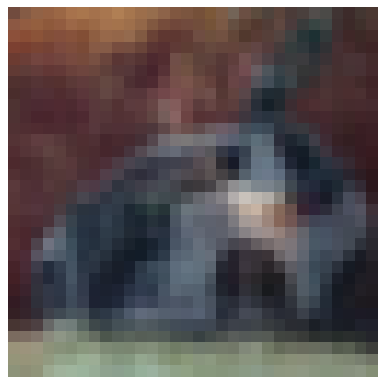
\includegraphics[width=0.3\textwidth]{images/mixup_example.png}
    \caption{}
\end{figure}

\newpage